%%%%%%%%%%%%%%%%%%%%%%%%%%%%%%%%%%%%%%%%%%%%%%%%%%%%%%%%%%%%%%%%%%%%%%%%%%%%%%%%
%                                                                              %
%            A Painless Introduction to Programming UAMMD Modules              %
%                    Chapter 2: Unleash your own potential                     %
%                                                                              %
%                          Marc Meléndez Schofield                             %
%                                                                              %
%%%%%%%%%%%%%%%%%%%%%%%%%%%%%%%%%%%%%%%%%%%%%%%%%%%%%%%%%%%%%%%%%%%%%%%%%%%%%%%%

You can only have so much fun playing with a Lennard-Jones simulation. Changing
the parameter values and then looking for differences in your plots gets old
soon. If you have made it this far, you want more. You imagine molecules, or
larger structures. Perhaps you would like to simulate billowing smoke, sloshing
water, or planets orbiting a star. All in good time.

Whatever your final aim, you need new interactions, and this chapter contains a
good collection of them.

\section{Harmonic bonds}

The simplest permanent link between particles in UAMMD has to be the harmonic
bond. Think of it as an invisible linear spring connecting two particles. As
long as they remain at the equilibrium distance $r_0$, they exert no force on
each other, but when you stretch their separation $r$, they pull back. The
potential function for this bond, then, equals
\begin{equation*}
  V(r) = \frac{1}{2}\ k\ (r - r_0)^2,
\end{equation*}
where the spring constant $k$ quantifies the bond rigidity.

Take a string of one hundred and one particles as our explanatory device. We
will line them all up along a curved queue, standing initially at rest.
\label{stringInitialConditions}
\begin{lstlisting}
%! codeblock: stringInitialConditions
  int numberOfParticles = 101;
  auto particles
    = make_shared<ParticleData>(numberOfParticles, sys);

  {
    auto position
      = particles->getPos(access::location::cpu,
                          access::mode::write);
    auto velocity
      = particles->getVel(access::location::cpu,
                          access::mode::write);

    real amplitude = 0.1;
    real stringlength = 1.0;
    int modenum = 1;
    for(int i = 0; i < numberOfParticles; ++i) {
      position[i].x = i*(stringlength/(numberOfParticles - 1));
      position[i].y = amplitude*sin(modenum*M_PI*position[i].x);
      position[i].z = position[i].w = 0;
      velocity[i].x = velocity[i].y = velocity[i].z = 0;
    }
  }
%! codeblockend
\end{lstlisting}

UAMMD reads bond information in from an external file. Let me first explain the
format of this plain text bond file. It should look something like this:
\begin{lstlisting}
100
0 1 1000.0 0.01
1 2 1000.0 0.01
2 3 1000.0 0.01
3 4 1000.0 0.01
    . . .
\end{lstlisting}
and so on. The file begins with the number of bonds ($100$) followed by a row
for each bond presenting $i$, $j$, $k$ and $r_0$, that is, the particle ID
numbers, the bond spring constant and the equilibrium distance. Hence, the next
line links particles $0$ and $1$ with a bond of $k = 1000.0$ and $r_0 = 0.01$.
After that, we get the values for the bond connecting particles $1$ and $2$.
Even though I have chosen identical values of $k$ and $r_0$ for all the bonds in
this example, you can of course make them all different if you like.

In addition to linking particles, you can attach them to fixed points in space.
We will pin particle $0$ to the origin of coordinates and particle $100$ to
point $(1, 0, 0)$. After the previous list of bonds, we must include the number
of fixed bonds (only $2$ in our case). The format for these is simply $i$, $x$,
$y$, $z$, $k$, $r_0$, meaning: particle ID, position in space $(x, y, z)$,
spring constant and equilibrium distance. So in our example, the bond file
should end with:
\begin{lstlisting}
2
0 0 0 0 1000.0 0.0
100 1 0 0 1000.0 0.0
%!
\end{lstlisting}
With the ends held in place, we have a taut string. As soon as we let go and run
the simulation, it should vibrate.

We will make the program write the bond information so that we don't have to.
\begin{lstlisting}
%! codeblock: stringBondFile
  {
    std::ofstream bondInfo("data.bonds");
    if(not bondInfo.is_open()) {
      sys->log<System::CRITICAL>("Unable to create data.bonds file. Halting program.");
      exit(-1);
    }

    bondInfo<<(numberOfParticles - 1)<<endl;
    for(int i = 0; i < numberOfParticles - 1; ++i) {
      bondInfo<<i<<" "<<(i + 1)<<" 1000.0 0.01"<<endl;
    }
    bondInfo<<"2"<<endl;
    bondInfo<<"0 0 0 0 1000.0 0.0"<<endl;
    bondInfo<<"100 1 0 0 1000.0 0.0"<<endl;
  }
%! codeblockend
\end{lstlisting}

Including the bonds presents no difficulties from the point of view of UAMMD
code, as the code resembles the lines we wrote for the Lennard-Jones
interaction. You insert the customary include at the top,
\begin{lstlisting}
# include "Interactor/BondedForces.cuh"
%!
\end{lstlisting}
define the interaction parameters to create the ``interactor'',
\begin{lstlisting}
%! codeblock: stringBondInteractor
  {
    using HarmonicBonds = BondedForces<BondedType::Harmonic>;
    HarmonicBonds::Parameters bondParameters;
    bondParameters.file = "data.bonds";
    auto bonds = make_shared<HarmonicBonds>(particles, sys, bondParameters);
%! codeblockend
\end{lstlisting}
and then add the new bond interaction to the integrator.
\begin{lstlisting}
%! codeblock: stringAddInteractor
    integrator->addInteractor(bonds);
  }
%! codeblockend
\end{lstlisting}

To replicate the simulation results shown in Figure \ref{vibratingString},
set the integrator parameters to these values:
\begin{lstlisting}
%! codeblock: VerletParameters
  using Verlet = VerletNVE;
  Verlet::Parameters VerletParams;
  VerletParams.dt = 0.001;
  VerletParams.initVelocities=false;
%! codeblockend
\end{lstlisting}
For the figure, I simulated twenty thousand steps and output the positions every
two thousand. Because I did not need a simulation box in this case, I eliminated
the corresponding block of code and changed the output command.
\begin{lstlisting}
      out<<endl;
      for(int id = 0; id < numberOfParticles; ++id)
        out<<position[index[id]]<<endl;
%!
\end{lstlisting}

\begin{comment}
Vibrating string simulation code:
\begin{lstlisting}
%! codefile: code/vibratingString.cu
# include "uammd.cuh"
# include "utils/InitialConditions.cuh"
# include "Interactor/BondedForces.cuh"
# include "Integrator/VerletNVE.cuh"

using namespace uammd;
using std::make_shared;
using std::endl;

int main(int argc, char *argv[]){

  auto sys = make_shared<System>(argc, argv);

  %! codeinsert: stringInitialConditions

  %! codeinsert: VerletParameters

  %! codeinsert: Verlet src: chapters/first_simulation.tex

  %! codeinsert: stringBondFile

  %! codeinsert: stringBondInteractor

  %! codeinsert: stringAddInteractor

  std::string outputFile = "vibratingString.dat";
  std::ofstream out(outputFile);

  int numberOfSteps = 20000;
  int printEverynSteps = 2000;

  for(int step = 0; step < numberOfSteps; ++step) {
    integrator->forwardTime();

    if(printEverynSteps > 0
       and step % printEverynSteps == 1) {
      auto position
        = particles->getPos(access::location::cpu,
                            access::mode::read);
      const int * index = particles->getIdOrderedIndices(access::location::cpu);

      out<<endl;
      for(int id = 0; id < numberOfParticles; ++id)
        out<<position[index[id]]<<endl;
    }
  }

  sys->finish();

  return 0;
}
%! codeend
\end{lstlisting}
\end{comment}

\begin{figure}
  \centering
  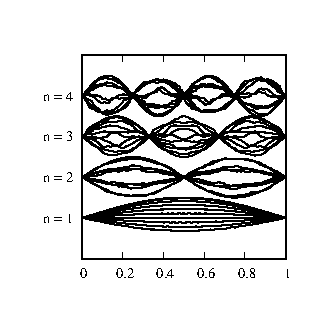
\includegraphics[width = 0.6 \textwidth]{figures/vibratingString.eps}
  \caption{\label{vibratingString}A chain of $101$ particles connected with
           harmonic bonds and ends tethered to fixed points. It (imperfectly)
           follows the behaviour of the ideal vibrating string. The first four
           normal modes of vibration were achieved by setting the
           \texttt{modenum} variable (see page
           \pageref{stringInitialConditions}) to $n = 1, 2, 3,$ and $4$.}
\end{figure}

\section{External fields}

Figure \ref{vibratingString} may hold the attention of harmonic analysis
enthusiasts but, personally, I cannot wait to free the chain of particles at one
end and simulate a hanging rope. We already know how to deal with the bonds. We
just eliminate the final fixed bond in the data.bonds file, leaving the end of
the file like this:
\begin{lstlisting}
1
0 0 0 0 1000.0 0.0
%!
\end{lstlisting}

GRAVITY.

\begin{figure}
  \centering
  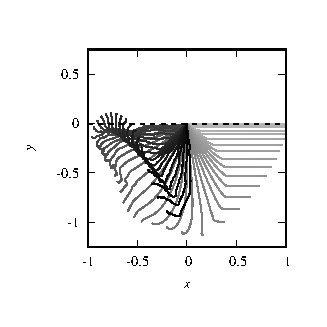
\includegraphics[width = 0.6 \textwidth]{figures/swingingRope.eps}
  \caption{\label{swingingRope}A chain of $101$ particles connected with
           harmonic bonds attached to the origin behaves like a swinging rope
           in a gravitational field.}
\end{figure}


\section{Alternative types of bonds}

FENE

Fixed bonds

Angular bonds

Torsional bonds

\section{Classical orbits}

\section{Defining your own potentials}

Bond potentials

Pair interactions
